\documentclass[11pt,a4paper]{article}

\usepackage[T1]{fontenc}
\usepackage[utf8]{inputenc}
\usepackage{lmodern}
\usepackage{amsmath}
\usepackage{amssymb}
\usepackage{textcomp}
\usepackage[margin=2.4cm]{geometry}
\usepackage{booktabs}
\usepackage{array}
\usepackage{xcolor}
\usepackage{enumitem}
\usepackage{tikz}
\usetikzlibrary{arrows.meta,positioning,calc}
\usepackage{fancyhdr}
\usepackage{titlesec}
\usepackage[hidelinks]{hyperref}

\definecolor{bodark}{HTML}{111827}
\definecolor{boaccent}{HTML}{2563EB}
\definecolor{bomuted}{HTML}{6B7280}
\definecolor{bosoft}{HTML}{EEF2FF}

\titleformat{\section}{\Large\bfseries\color{bodark}}{\thesection}{0.6em}{}
\titleformat{\subsection}{\large\bfseries\color{bodark}}{\thesubsection}{0.6em}{}
\titlespacing*{\section}{0pt}{1.6em}{0.6em}

\pagestyle{fancy}
\fancyhf{}
\fancyhead[L]{\small\color{bomuted}BO --- Business Command Center}
\fancyhead[R]{\small\color{bomuted}\thepage}
\renewcommand{\headrulewidth}{0.4pt}

\newcommand{\term}[1]{\textcolor{boaccent}{\textbf{#1}}}
\newcommand{\eur}{\texteuro}

\newsavebox{\calloutbox}
\newenvironment{callout}%
{\begin{center}\begin{lrbox}{\calloutbox}\begin{minipage}{\dimexpr0.94\textwidth-24pt\relax}\color{bodark}}%
{\end{minipage}\end{lrbox}\setlength{\fboxsep}{12pt}\colorbox{bosoft}{\usebox{\calloutbox}}\end{center}}

\title{\vspace{-1.5cm}\textbf{\Huge BO}\\[0.4em]
  \large An AI-native Business Command Center\\[0.25em]
  \normalsize\color{bomuted}Platform architecture, the self-improving data loop, and a business model}
\author{}
\date{\small\today}

\begin{document}
\maketitle
\thispagestyle{fancy}

\begin{abstract}
\noindent
BO turns one sentence about a company into a working administration platform. Instead of shipping
every business system and asking the operator to switch off what they do not need, BO researches the
company, decides what it actually runs on, and builds only that. Every company that uses BO leaves
behind anonymous evidence about how its industry really operates, and that evidence --- not an
opinion held by BO's authors --- decides what the next company in the same industry is given. The
product therefore becomes more accurate as it is used, and the accuracy compounds per industry
rather than per customer. This document describes BO as a platform, describes the data loop that
improves it, and sets out a business model built on top of both.
\end{abstract}

\section{The problem}

Enterprise administration software is priced and shaped for the largest customer it can find. Odoo,
Microsoft Dynamics, SAP Business One, NetSuite and Salesforce all solve it the same way: ship every
module, then make configuration the buyer's problem. The consequences are consistent across all of
them.

\begin{itemize}[leftmargin=1.4em,itemsep=2pt]
  \item \textbf{Bloat.} A suite offers forty or more modules. A mid-sized company uses a handful.
        The rest is navigation the operator must learn to ignore.
  \item \textbf{Implementation cost.} The software is not the purchase; the consultant who shapes it
        is. Implementation routinely costs several multiples of licence spend, and takes months.
  \item \textbf{Wrong default shape.} The system is built around a generic large-enterprise process.
        A three-person plumbing business is asked to think in opportunities, quote lines and business
        partner masters.
  \item \textbf{The all-or-nothing trap.} Smaller companies escape by running eight disconnected
        tools --- a payment processor, an accounting package, a CRM, a spreadsheet, a scheduling app
        --- and rekeying between them.
\end{itemize}

The gap is real: between \emph{one spreadsheet} and \emph{a six-month ERP implementation} there is
almost nothing. BO is aimed exactly there.

\section{BO as a platform}

\subsection{The core claim}

The operator describes the business in ordinary language. BO returns a \term{Command Center}: a
working administration platform containing only the systems that business runs on, with its own
record types, views, metrics and workflows.

\begin{callout}
\textbf{Design rule.} BO installs \emph{structure}, never fiction. A generated workspace contains
record types, relationships, views and workflows. It never contains invented customers, invented
transactions, invented employees or invented performance figures. An empty Command Center is
correct; a plausible-looking fake one is not.
\end{callout}

\subsection{The build pipeline}

\begin{center}
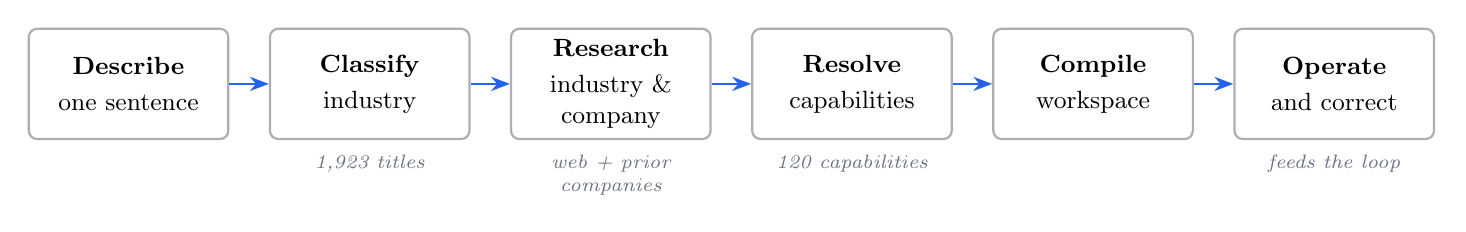
\begin{tikzpicture}[
  node distance=0.5cm,
  stage/.style={rectangle, rounded corners=3pt, draw=bodark!35, fill=white, thick,
                text width=2.3cm, align=center, minimum height=1.4cm, font=\small},
  lbl/.style={font=\scriptsize\itshape, text=bomuted, text width=2.4cm, align=center},
  arr/.style={-{Stealth[length=2.4mm]}, draw=boaccent, thick}
]
\node[stage] (s1) {\textbf{Describe}\\[2pt] one sentence};
\node[stage, right=of s1] (s2) {\textbf{Classify}\\[2pt] industry};
\node[stage, right=of s2] (s3) {\textbf{Research}\\[2pt] industry \& company};
\node[stage, right=of s3] (s4) {\textbf{Resolve}\\[2pt] capabilities};
\node[stage, right=of s4] (s5) {\textbf{Compile}\\[2pt] workspace};
\node[stage, right=of s5] (s6) {\textbf{Operate}\\[2pt] and correct};

\foreach \a/\b in {s1/s2, s2/s3, s3/s4, s4/s5, s5/s6} \draw[arr] (\a) -- (\b);

\node[lbl, below=2pt of s2] {1{,}923 titles};
\node[lbl, below=2pt of s3] {web + prior companies};
\node[lbl, below=2pt of s4] {120 capabilities};
\node[lbl, below=2pt of s6] {feeds the loop};
\end{tikzpicture}
\end{center}

\begin{enumerate}[leftmargin=1.6em,itemsep=3pt]
  \item \textbf{Describe.} A sentence, in the operator's own words.
  \item \textbf{Classify.} The sentence is matched against a 1{,}923-title industry taxonomy using
        rarity-weighted lexical evidence pooled per subsector, so a rare distinguishing word
        (``quarry'', ``retainer'') counts for far more than a common one (``customers'').
  \item \textbf{Research.} Two tiers. A small model running in the browser resolves the obvious.
        Where the answer genuinely matters and is genuinely unknown, a frontier model researches the
        open web and returns cited conclusions.
  \item \textbf{Resolve.} Selected capabilities pull in their dependencies and prune what has become
        unreachable. Invoicing cannot exist without something to invoice.
  \item \textbf{Compile.} Capabilities compile into entities, navigation, views, metrics, workflows
        and role permissions --- a versioned project with rollback.
  \item \textbf{Operate.} The operator uses it, and corrects it. Those corrections are the input to
        Section~\ref{sec:loop}.
\end{enumerate}

\subsection{Asking fewer, better questions}

BO models a business along seven operating dimensions: what it \emph{offers}, how it takes
\emph{revenue}, how it \emph{delivers}, who its \emph{customer} is, how its \emph{workforce} is
organised, whether it has a physical \emph{supply} chain, and what \emph{control} obligations it
carries. Some dimensions are marked essential; a business cannot be built without resolving them.

Each candidate question is scored by \term{information gain} --- how much of the still-undecided
workspace its answer would settle:
\[
  \mathrm{gain}(d) \;=\; w_d \times \bigl(1 + \lvert C_{\text{undecided}}(d)\rvert\bigr)
\]
where $w_d$ is the dimension's weight and $C_{\text{undecided}}(d)$ the set of capabilities whose
inclusion still turns on $d$. BO asks the highest-gain unresolved question, and stops once nothing
left to ask would change the outcome. Discovery is short because most questions are not worth
asking.

\subsection{Where an answer comes from}

Every decision BO makes carries its \term{basis} --- the reason BO believes it. Bases are ranked,
and a stronger basis always overrides a weaker one.

\begin{center}
\begin{tabular}{@{}c l l@{}}
\toprule
\textbf{Rank} & \textbf{Basis} & \textbf{Meaning} \\
\midrule
1 & \texttt{stated}              & The operator said so. Nothing overrides this. \\
2 & \texttt{researched}          & Found about \emph{this} company, with sources. \\
3 & \texttt{observed}            & What other companies in this industry actually did. \\
4 & \texttt{industry-researched} & What research found about the industry, with sources. \\
5 & \texttt{domain-default}      & BO's own rules. Never selects a system on its own. \\
\bottomrule
\end{tabular}
\end{center}

Ranks 3 and 4 are the subject of Section~\ref{sec:loop}, and they are what makes BO improve with
use.

\subsection{The knowledge base}

\begin{center}
\begin{tabular}{@{}l l l@{}}
\toprule
\textbf{Layer} & \textbf{Contents} & \textbf{Origin} \\
\midrule
Industry taxonomy    & 20 sectors, 96 subsectors, 1{,}923 titles & NAICS 2022 (public domain) \\
Operating archetypes & 25 packs mapping industry to systems      & Authored \\
Capability catalog   & 120 buildable business systems            & Authored \\
Industry evidence    & Per-industry research and observations    & \textbf{Earned from use} \\
\bottomrule
\end{tabular}
\end{center}

Only the taxonomy is imported, and deliberately so. It is public domain, and it solves the one
problem that cannot be authored: enumerating every kind of business that exists, in the vocabulary
operators use about themselves. Vendor data models from commercial ERP products are copyrighted and
are not used; they would also be the wrong input, since they describe another product's menus rather
than a company's needs.

\begin{callout}
\textbf{A taxonomy classifies; it does not explain.} The taxonomy can tell BO that a company is an
advertising agency. It contains no fact about whether advertising agencies bill by the hour. That
gap is precisely why the layer in Section~\ref{sec:loop} exists.
\end{callout}

\subsection{Measured differentiation}

The platform's central claim is that different companies get genuinely different systems. The table
below is produced by the live planner, not written by hand.

\begin{center}
\small
\begin{tabular}{@{}l c c p{6.9cm}@{}}
\toprule
\textbf{Company described} & \textbf{Pages} & \textbf{Modules} & \textbf{Examples of what only it gets} \\
\midrule
Trucking / freight & 12 & 9  & Fleet, Shipping, Equipment \\
B2B SaaS           & 15 & 9  & Subscriptions, Customer success, Knowledge base, Lead sources \\
Marketing agency   & 10 & 7  & Projects, Tasks, Retainers, Documents \\
Restaurant         & 14 & 10 & Point of sale, Reservations, Shifts, Suppliers \\
Manufacturer       & 18 & 11 & Bills of materials, Production, Lots and serials, Warehouses \\
\bottomrule
\end{tabular}
\end{center}

Every company receives the same six-item shell --- Home, Today, Analytics, Links, Assistant,
Settings. Everything between those differs. A regression test asserts that no two of these companies
can ever receive an identical set of pages, and that operations-heavy businesses must each hold at
least three page types no other business receives. That test exists because a planner quietly
collapsing to one generic base would pass every other test in the system while destroying the entire
reason the product exists.

\subsection{Connected apps}

BO does not attempt to replace the systems of record a company already trusts. Payment processing,
statutory accounting and payroll are regulated, deeply integrated, and better solved by incumbents.

Instead BO connects to them and presents them in one place, under a strict contract:

\begin{itemize}[leftmargin=1.4em,itemsep=2pt]
  \item \textbf{Read is the default.} Connected data is shown, linked and reported on.
  \item \textbf{Writes are explicit, queued and idempotent.} Every write carries a stable
        idempotency key, passes through an outbox, and retries a bounded number of times before
        being abandoned visibly rather than silently.
  \item \textbf{Conflicts are never merged.} If a record moved on both sides, BO stops and shows the
        operator both versions. Silent reconciliation of financial data is not acceptable.
\end{itemize}

This turns BO's weakest position --- being new, and therefore not yet anyone's system of record ---
into its most useful one: the single surface across everything the company already runs.

\section{The self-improving data loop}
\label{sec:loop}

\subsection{Why BO cannot simply be authored}

Consider a concrete question: \emph{does a social media agency need timesheets?}

No dataset answers it. The taxonomy classifies the agency and says nothing about how it bills.
Whoever authored BO's rules would have to guess --- and a vendor's guess, applied to every customer
in an industry, is exactly the failure that makes existing suites feel wrong. Asking the customer
only moves the guess; a new operator often does not know either.

The only credible answer is evidence. BO therefore learns per industry, from two sources, and the
answer improves as more companies pass through.

\subsection{Two sources of evidence}

\begin{center}
\begin{tabular}{@{}l p{5.0cm} p{5.0cm}@{}}
\toprule
 & \textbf{Researched} & \textbf{Observed} \\
\midrule
What it is   & A frontier model researches the industry on the open web, with citations. & What real companies in the industry did with the workspace BO gave them. \\
When         & Once per industry; the first company in it triggers the pass. & Continuously, as companies keep, remove or add systems. \\
Who benefits & Every later company in that industry. & Every later company in that industry. \\
Strength     & Good cold start. Can be wrong or dated. & Ground truth. Slow to accumulate. \\
\bottomrule
\end{tabular}
\end{center}

\term{Observation outranks research, and research outranks BO's own rules.} What companies actually
do beats what an article says about them. Research speaks only where behaviour is still silent.

\subsection{The loop}

\begin{center}
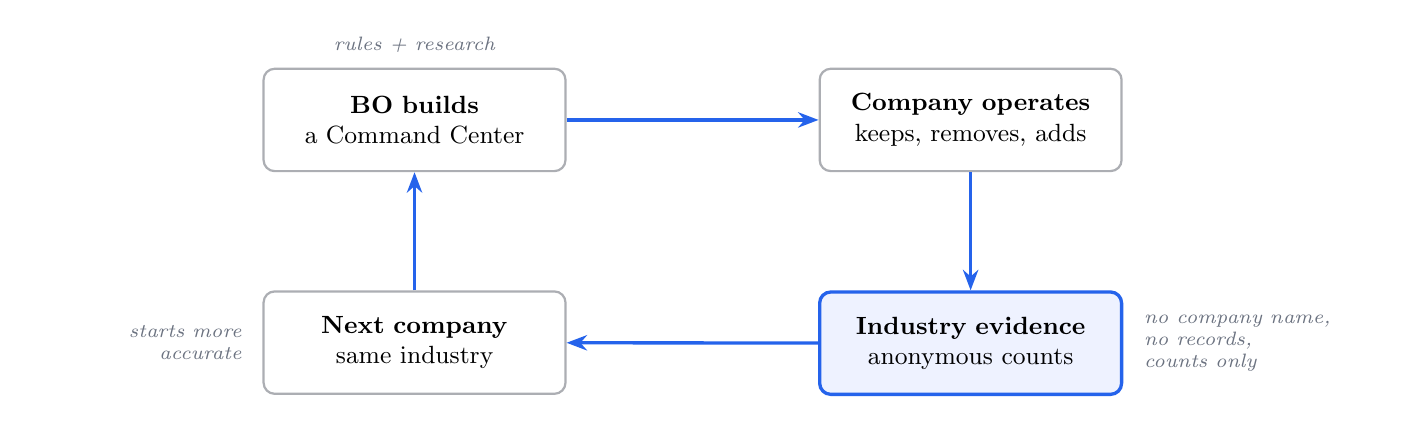
\begin{tikzpicture}[
  node distance=1.5cm and 3.2cm,
  box/.style={rectangle, rounded corners=4pt, draw=bodark!35, fill=white, thick,
              text width=3.6cm, align=center, minimum height=1.3cm, font=\small},
  ev/.style={rectangle, rounded corners=4pt, draw=boaccent, fill=bosoft, very thick,
             text width=3.6cm, align=center, minimum height=1.3cm, font=\small},
  arr/.style={-{Stealth[length=2.6mm]}, draw=boaccent, very thick},
  note/.style={font=\scriptsize\itshape, text=bomuted}
]
\node[box] (build) {\textbf{BO builds}\\a Command Center};
\node[box, right=of build] (use) {\textbf{Company operates}\\keeps, removes, adds};
\node[ev, below=of use] (store) {\textbf{Industry evidence}\\anonymous counts};
\node[box, below=of build] (next) {\textbf{Next company}\\same industry};

\draw[arr] (build) -- (use);
\draw[arr] (use) -- (store);
\draw[arr] (store) -- (next);
\draw[arr] (next) -- (build);

\node[note, above=2pt of build, text width=3.6cm, align=center] {rules + research};
\node[note, right=4pt of store, text width=3.0cm] {no company name,\\no records,\\counts only};
\node[note, left=4pt of next, text width=2.6cm, align=right] {starts more\\accurate};
\end{tikzpicture}
\end{center}

Each turn of the loop makes the next build in that industry more accurate. The loop closes without
any human deciding anything.

\subsection{Guards, because bad learning is worse than none}

A system that learns the wrong thing confidently is more dangerous than one that does not learn. The
mechanism is therefore deliberately conservative.

\begin{center}
\begin{tabular}{@{}l p{9.0cm}@{}}
\toprule
\textbf{Guard} & \textbf{What it prevents} \\
\midrule
Minimum five companies    & One opinionated operator speaking for a whole industry. \\
Sixty per cent threshold  & A narrow majority changing what everyone is given. \\
Splits stay undecided     & Five keep against five remove yields \emph{no} verdict, not a coin flip. \\
Counted per company       & A busy operator clicking repeatedly outvoting an industry. \\
Aggregates only           & Any leakage of company identity, records or content. \\
Input validated           & Malformed or hostile identifiers ever reaching storage. \\
Reason attached           & Unexplainable behaviour. Every verdict states its own evidence. \\
\bottomrule
\end{tabular}
\end{center}

The reason is surfaced to the operator directly, in the build journal:

\begin{callout}
\textbf{What six other professional services companies actually kept.}\\
BO is not guessing here. Three of these decisions come from what real companies in this industry did
with the workspace BO built them.
\end{callout}

\subsection{Privacy by construction}

Only counts leave a workspace. The stored record for an industry has the form ``for capability
\texttt{work.time}: kept 2, removed 6, added 0; eight companies contributing''. There is no company
name, no workspace identifier, no record and no field content. A test searches the persisted files
to assert that no identifying token can appear in them. Companies contribute to their industry's
knowledge without contributing anything about themselves.

\subsection{Why this compounds}

\begin{itemize}[leftmargin=1.4em,itemsep=3pt]
  \item \textbf{The unit of learning is the industry, not the customer.} A hundred customers spread
        across five industries produce five well-calibrated industries, not a hundred lightly-tuned
        accounts. Accuracy therefore arrives far earlier than customer count alone would suggest.
  \item \textbf{Research cost is paid once and shared.} The first restaurant in an industry pays for
        that industry's research. The thousandth inherits it at zero marginal cost.
  \item \textbf{Corrections are free labelled data.} An operator removing a page is not a churn
        signal to be mourned --- it is a clean label, produced during work the operator wanted to do
        anyway.
  \item \textbf{It cannot be copied by feature parity.} A competitor can clone BO's capability
        catalog in weeks. They cannot clone the record of what tens of thousands of real companies
        did with theirs. The moat is the loop, not the catalog.
  \item \textbf{Free users are an asset, not a cost.} A non-paying company still contributes
        evidence that improves what paying companies in its industry receive. This inverts the usual
        freemium calculus.
\end{itemize}

\begin{callout}
\textbf{Honest limit.} The loop starts empty. With no users there is no observed evidence, and BO
falls back to authored rules --- exactly the behaviour it exists to replace. The researched half can
be populated immediately, one pass per industry, but observation must be earned. The mechanism is
built, tested and live; the evidence has to accumulate.
\end{callout}

\section{BO as a business}

\subsection{Who it is for}

The wedge is the company that has outgrown spreadsheets and cannot justify an ERP implementation:
roughly five to two hundred employees, operationally real, with no dedicated systems administrator.
Within that, BO is strongest where operations are \emph{specific} --- field service, trades,
logistics, studios, clinics, small manufacturers --- because that is where generic suites feel most
wrong and where BO's differentiation is visible on day one.

\subsection{Positioning}

\begin{center}
\small
\begin{tabular}{@{}l p{4.2cm} p{6.0cm}@{}}
\toprule
\textbf{Category} & \textbf{Examples} & \textbf{How BO differs} \\
\midrule
Full ERP suites     & SAP, Dynamics, NetSuite, Odoo & They ship everything and charge to configure it. BO builds only what is needed, with no implementation project. \\
CRM-first platforms & Salesforce, HubSpot           & They treat the sales pipeline as the company. BO treats sales as one operating process among several. \\
Vertical SaaS       & ServiceTitan, Procore, Toast  & Excellent in one industry, absent from the rest. BO reaches any industry, and deepens per industry through the loop. \\
Build-your-own      & Airtable, Notion, Retool      & Flexible but blank. The operator must already know what to build. BO decides, then hands over something already correct. \\
\bottomrule
\end{tabular}
\end{center}

The defensible middle is the reach of a horizontal platform with the specificity of a vertical one,
achieved by \emph{learning} verticals instead of hand-building them.

\subsection{Why now}

Three things changed at once. Frontier models became capable of genuine research with citations
rather than plausible text. Small models became good enough to run discovery inside the browser at
zero marginal cost. And nearly every system of record a small company uses now exposes a usable API,
which is what makes the connected-apps layer possible at all.

\section{Business model}

\subsection{Revenue lines}

\begin{center}
\small
\begin{tabular}{@{}l l p{6.4cm}@{}}
\toprule
\textbf{Tier} & \textbf{Indicative price} & \textbf{Contents} \\
\midrule
\textbf{Free}       & \eur{}0
& One workspace, unlimited build and rebuild, local records, one connected app read-only.
  Contributes anonymous evidence. \\[3pt]
\textbf{Team}       & \eur{}19 per user / month
& Multiple users with roles, unlimited connected apps read-only, automations, versioned rollback,
  export. \\[3pt]
\textbf{Business}   & \eur{}39 per user / month
& Write-back to connected apps, on-demand frontier research for this company, audit history,
  priority rebuilds, support terms. \\[3pt]
\textbf{Enterprise} & from \eur{}15{,}000 / year
& Self-hosting, single sign-on, data residency, custom connectors, contracted support. \\
\bottomrule
\end{tabular}
\end{center}

Secondary lines, ordered by how far away they are:

\begin{enumerate}[leftmargin=1.6em,itemsep=3pt]
  \item \textbf{Usage-priced research.} A deep research pass on a specific question is metered,
        included in Business up to a quota.
  \item \textbf{Connector marketplace.} Third parties publish connectors against BO's write-back
        contract and BO takes a share. It doubles as distribution: every connector's vendor has a
        reason to send customers to BO.
  \item \textbf{Industry benchmarks.} The evidence store already holds anonymous, aggregated,
        per-industry operating patterns. These can be sold back to operators as ``how companies like
        yours run'' --- never as anything traceable to a company. This line becomes credible only at
        scale, and must never be allowed to compromise the privacy guarantees the loop depends on.
\end{enumerate}

\subsection{Unit economics}

Two costs matter, and both behave well.

\begin{center}
\begin{tabular}{@{}l l l@{}}
\toprule
\textbf{Cost} & \textbf{Behaviour} & \textbf{Direction with scale} \\
\midrule
Discovery model     & Runs in the browser.                    & Zero marginal cost, always. \\
Industry research   & Once per industry, then shared.         & Falls toward zero per customer. \\
Company research    & Optional, metered, on demand.           & Priced through, not absorbed. \\
Hosting and storage & Structured records; no media workload.  & Low and linear. \\
Connector upkeep    & Fixed per connector.                    & Amortised across all users of it. \\
\bottomrule
\end{tabular}
\end{center}

The structurally interesting property is that the largest AI cost --- research --- is incurred
\emph{per industry}, while revenue is collected \emph{per customer}. Gross margin therefore improves
as customers concentrate into industries already researched, which means sales effort focused on a
vertical improves margin and product accuracy at the same time.

\subsection{Go to market}

\begin{enumerate}[leftmargin=1.6em,itemsep=3pt]
  \item \textbf{Land through the free build.} The demonstration is the product: describe your
        company, watch a system specific to it appear in under a minute. Unusually easy to show, and
        unusually hard for a suite vendor to match.
  \item \textbf{Concentrate on a few verticals first.} Not because BO cannot reach the rest, but
        because concentration fills the evidence loop fastest, and one well-calibrated industry is a
        far stronger reference than a broad, shallow footprint.
  \item \textbf{Expand through connectors.} Each integration is both a retention hook and a
        co-marketing surface.
  \item \textbf{Move upmarket on trust.} Audit history, roles, self-hosting and data residency are
        what convert a working tool into a system of record.
\end{enumerate}

\subsection{Key metrics}

\begin{center}
\begin{tabular}{@{}l p{8.4cm}@{}}
\toprule
\textbf{Metric} & \textbf{What it tells you} \\
\midrule
Industries above threshold   & How much of the catalogue is evidence-backed rather than authored.
                               The best single proxy for compounding accuracy. \\
Corrections per build        & Should fall over time within an industry. If it does not, the loop is
                               not working. \\
Build to first record        & Whether the generated system was actually usable. \\
Connected apps per workspace & Depth of entrenchment; the strongest retention predictor. \\
Free to paid, by industry    & Whether accuracy converts, and which verticals to concentrate on. \\
\bottomrule
\end{tabular}
\end{center}

\section{Risks, stated plainly}

\begin{itemize}[leftmargin=1.4em,itemsep=3pt]
  \item \textbf{Cold start.} Before adoption, BO is only as good as its authored rules. Mitigation:
        run the researched pass across every target industry ahead of launch, and concentrate early
        sales so observation accumulates somewhere rather than thinly everywhere.
  \item \textbf{Observation bias.} Early adopters are not representative of their industries.
        Mitigation: the minimum-company threshold and the undecided-split rule, plus monitoring of
        whether verdicts drift as later, more typical companies arrive.
  \item \textbf{Connector maintenance.} Every integration is a permanent liability against an API BO
        does not control. Mitigation: a narrow, uniform write-back contract, and a marketplace so BO
        need not own every connector itself.
  \item \textbf{Trust as a system of record.} Companies are rightly conservative about where their
        operating data lives. Mitigation: export without lock-in, versioned rollback, conflict
        handling that never merges silently, and self-hosting for those who require it.
  \item \textbf{Incumbent response.} A suite vendor can add a natural-language setup wizard quickly.
        What they cannot easily do is \emph{narrow} their product: their pricing, their partner
        channel and their enterprise commitments all reward breadth. The asymmetry is commercial,
        not technical.
\end{itemize}

\section{Current state}

\begin{center}
\begin{tabular}{@{}l l@{}}
\toprule
\textbf{Component} & \textbf{Status} \\
\midrule
Industry taxonomy, 1{,}923 titles      & Built, tested \\
Capability catalog, 120 systems        & Built, integrity-tested \\
Discovery and information-gain planner & Built, tested \\
Workspace compiler and versioning      & Built, tested \\
Differentiation guarantee              & Built, regression-tested \\
Frontier research with citations       & Built; requires a provider key \\
Industry evidence loop                 & Built, tested; awaiting adoption to fill \\
Connected apps contract                & Built, tested; first live connector outstanding \\
\bottomrule
\end{tabular}
\end{center}

\vspace{1em}
\begin{callout}
\textbf{In one sentence.} BO is an administration platform that decides what a company needs instead
of asking it to configure what it does not --- and it decides better every time another company in
the same industry uses it.
\end{callout}

\end{document}
